Para la construcción del nodo 2, usaremos el siguiente cableado de la placa
Arduino Pro Mini:

%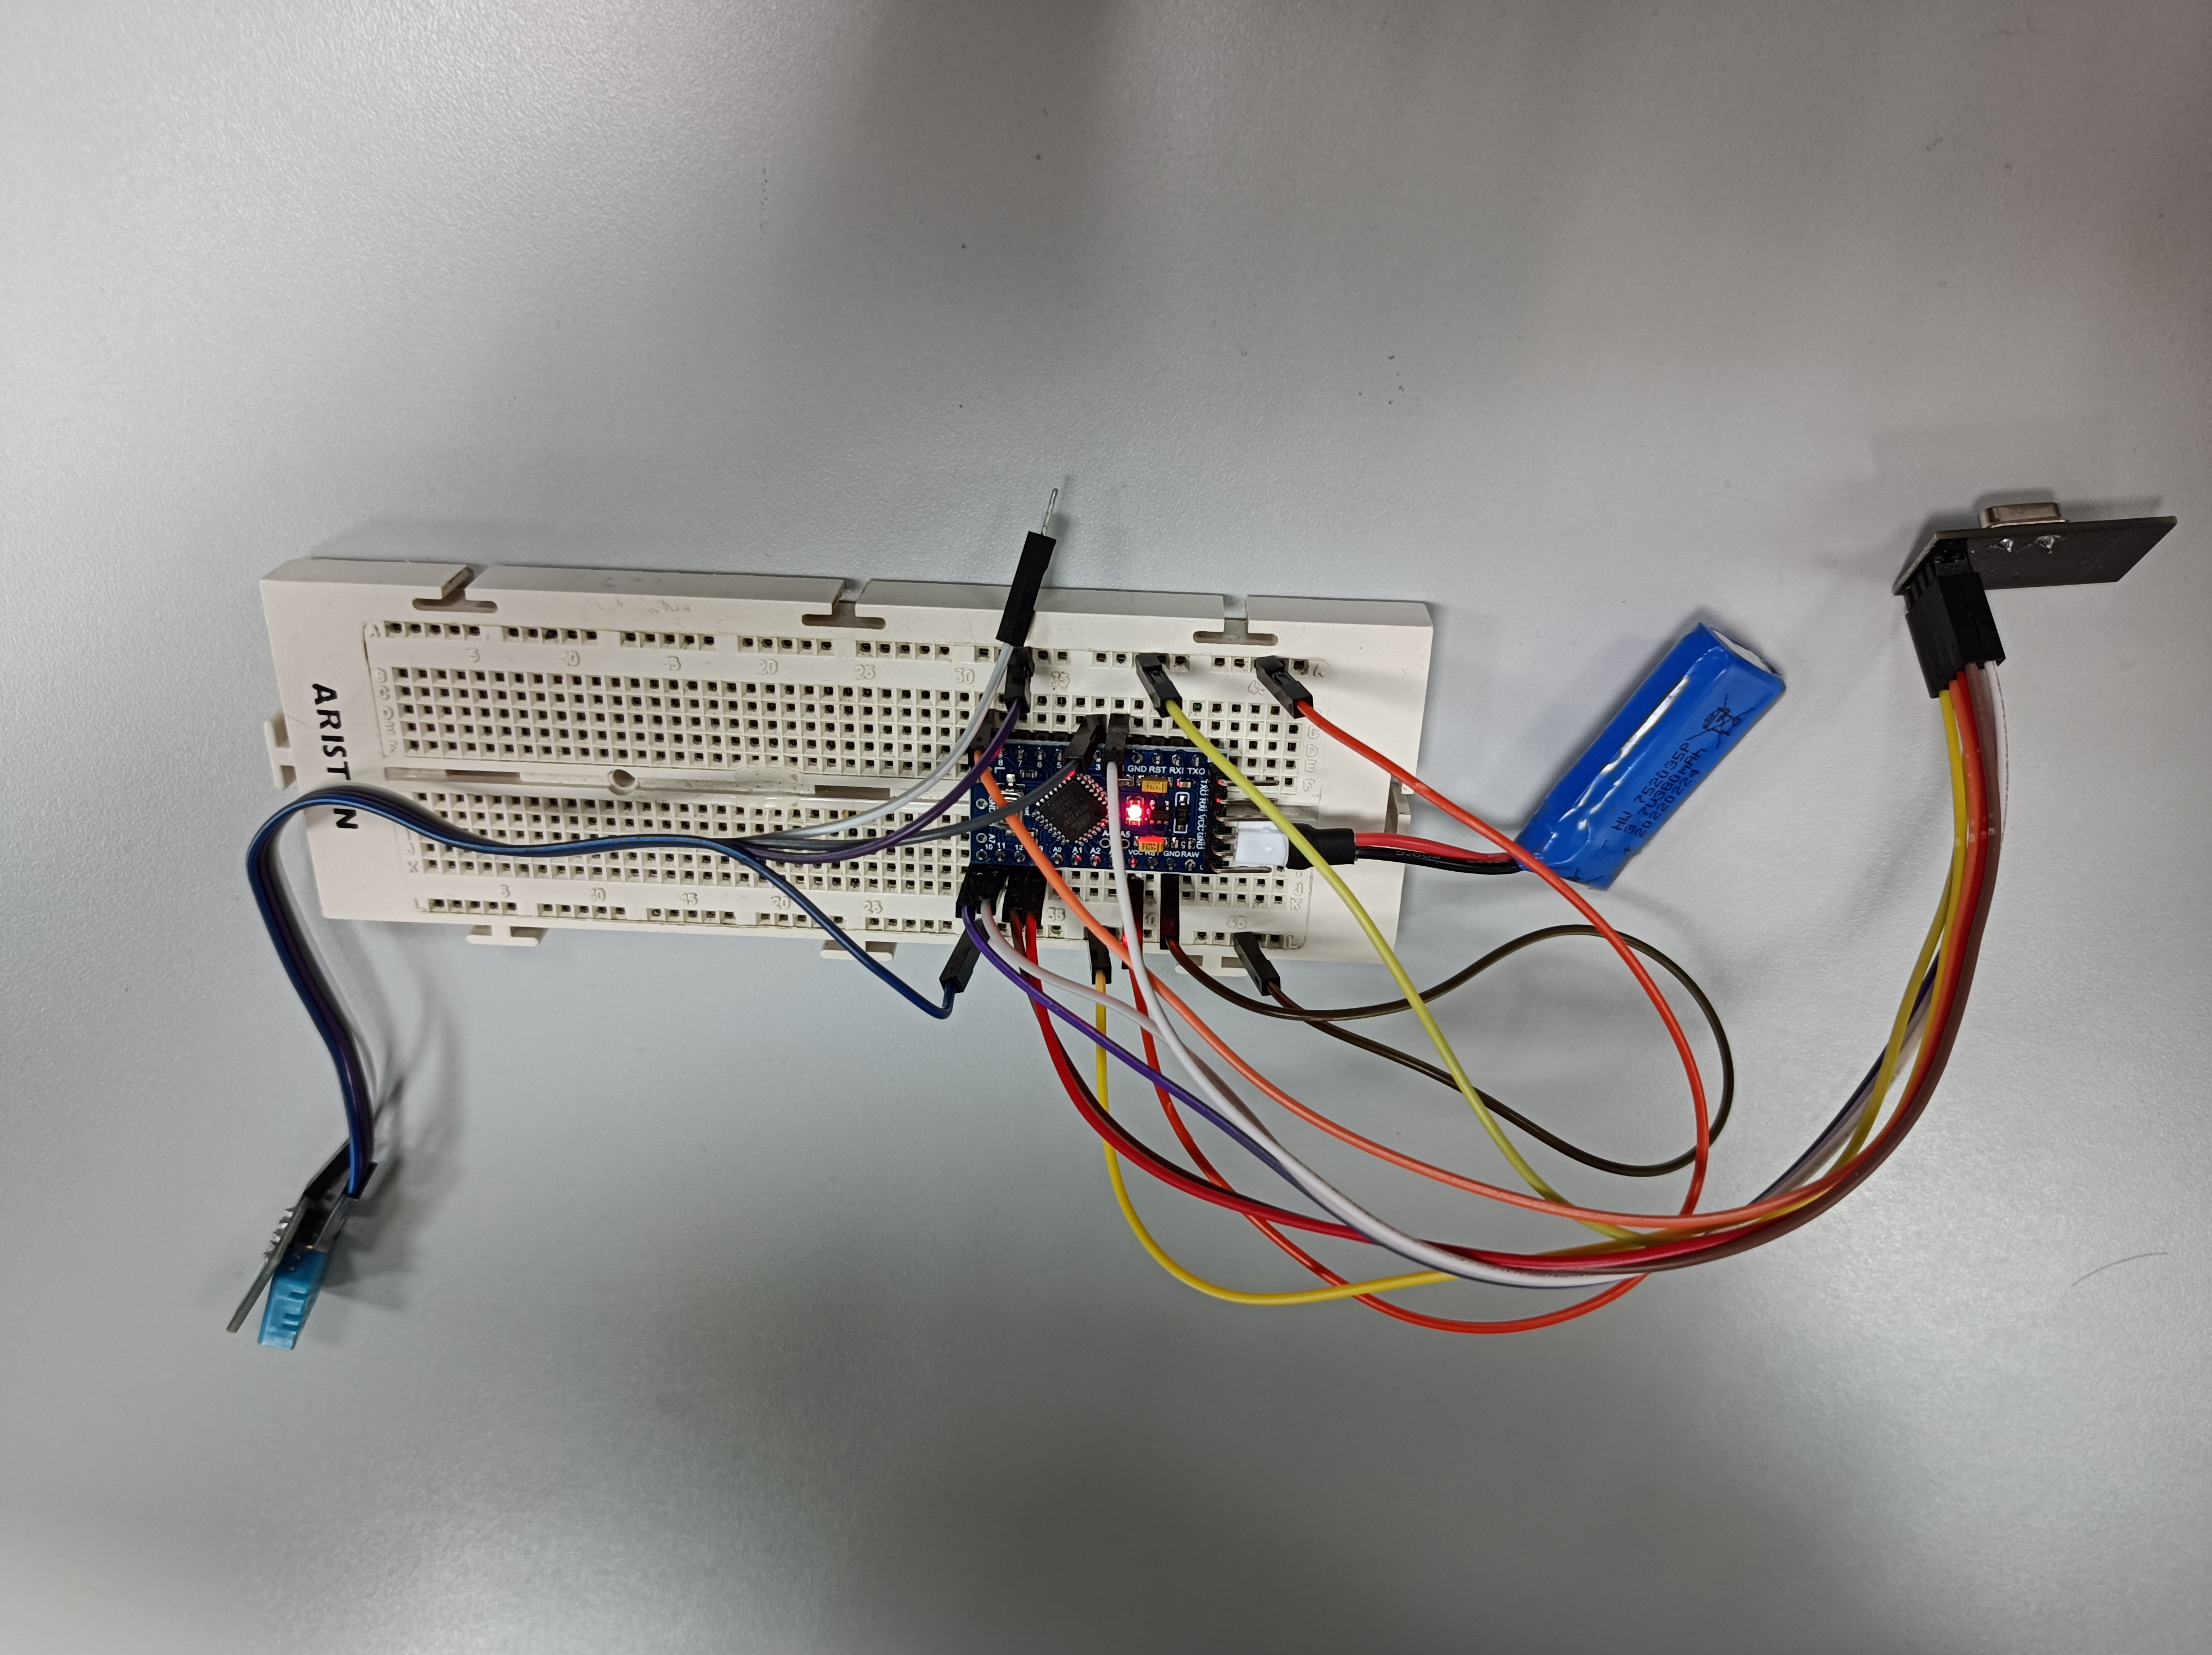
\includegraphics[width=\linewidth]{nodo2/nodo2-wiring.jpg}

Para la programación de la placa, además de la librería \emph{MySensors},
necesitamos las librerías \emph{arduino-DHT}\footnotemark y
\emph{Arduino\_Vcc}\footnotemark.

\footnotetext{\url{
    https://github.com/markruys/arduino-DHT/archive/cd24ce3ca32fe0caf05d6c21565c8d5605860a08.zip
}}
\footnotetext{\url{
    https://github.com/Yveaux/Arduino_Vcc/archive/2b2362b52e79ce102088c690e2bbcc595563c859.zip
}}

Usaremos este código:

\lstinputlisting[language=C++, caption=nodo2.ino]{2/nodo2/nodo2.ino}

En este caso, en el menú \emph{Configuración $\rightarrow$ Dispositivos} deberían
salir dos entradas con las lecturas de temperatura y humedad, y la del nivel
de batería:

%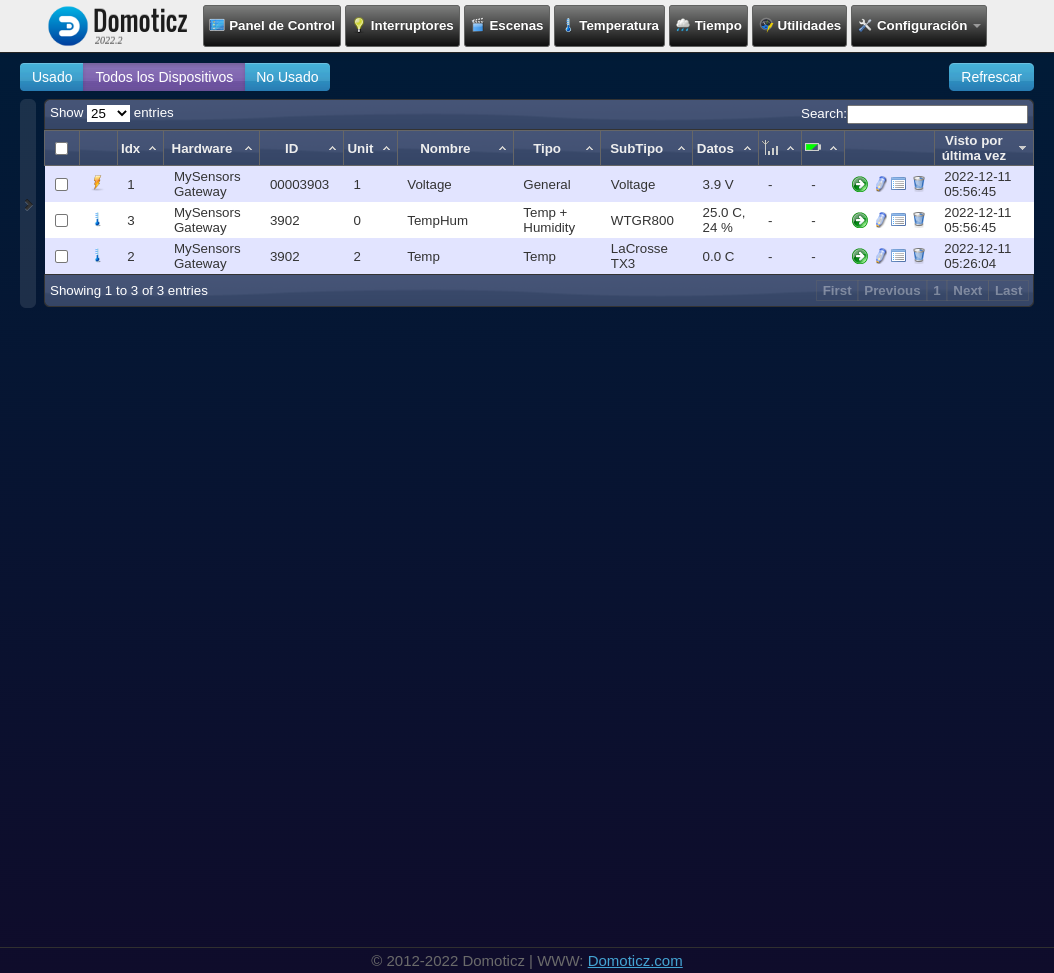
\includegraphics[width=\linewidth]{nodo2/nodo2-domoticz.jpg}